In order to complete this guide you will need the following equipment.

\begin{enumerate}
\item Laptop with the following: 
\begin{enumerate}
\item The \gls{sdr} Drivers. These are usually available from the manufacturers website.
\item The Arduino \gls{ide}\footnote{\url{https://www.arduino.cc/en/Main/Software}}.
\item The RadioHead-Extras library should be installed and made available to the Arduino IDE. The library is in the \verb|src| folder of this \gls{repo}.
\item gnuradio\footnote{\url{https://www.gnuradio.org}}.
\item A clone of this \gls{repo} and performed recursively\footnote{git clone --recursive https://github.com/geekskick/wex-guide}.
\end{enumerate}
\item An \gls{sdr} with an appropriate antenna for looking at the 430-440MHz frequency range. Its up to you which you use, there are loads available for a reasonable price\footnote{\url{https://www.rtl-sdr.com}}.
\item Two Adafruit Feathers with an RFM69 packet radio module attached\footnote{\url{https://learn.adafruit.com/adafruit-feather-m0-radio-with-rfm69-packet-radio/overview}} as shown in \cref{adafruit}. These should ideally have antennas attached as described in the Adafruit documentation\footnote{\url{https://learn.adafruit.com/adafruit-feather-m0-radio-with-rfm69-packet-radio/antenna-options}}. 

\centrefigurestart
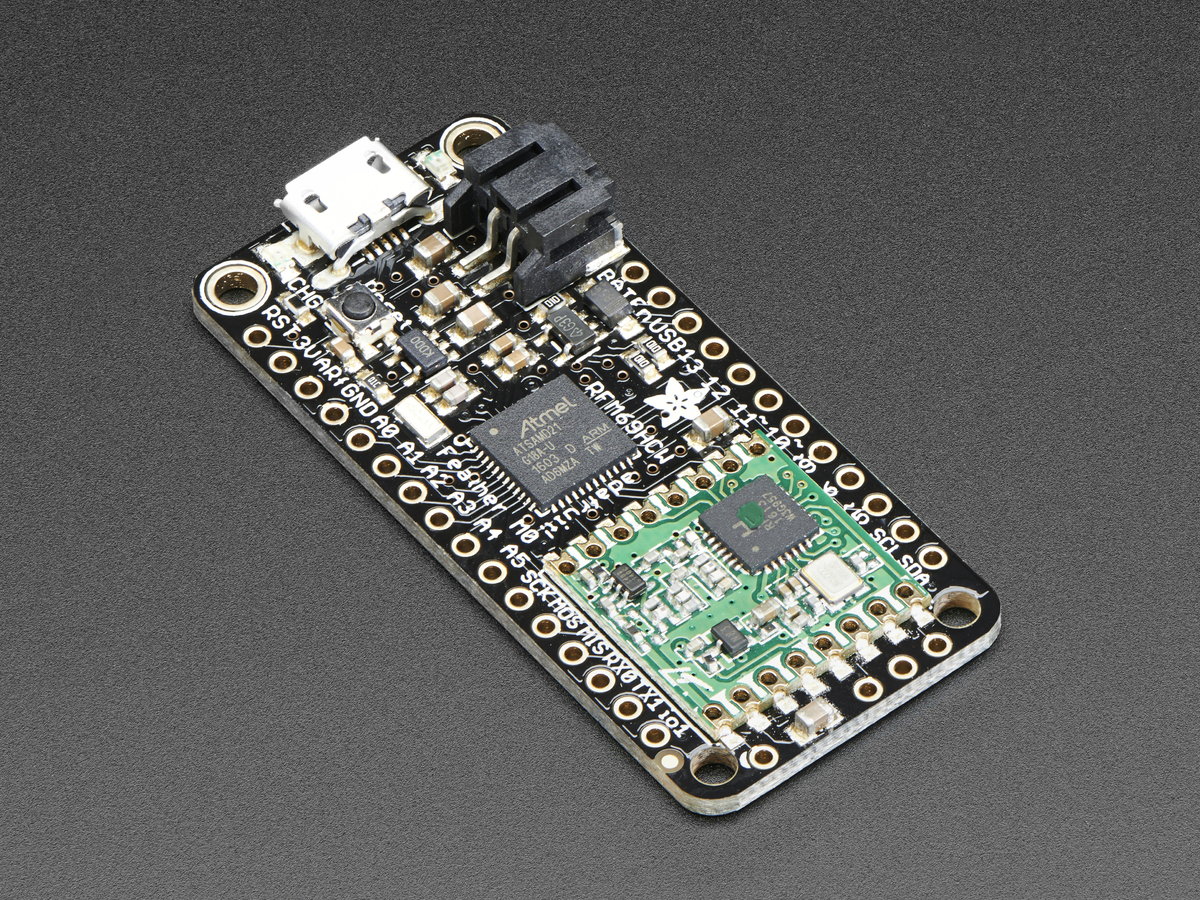
\includegraphics[width=\imgwidth]{feather.jpg}
\caption{An Adafruit Feather M0 with RFM69 Packet Radio}
\label{adafruit}
\centrefigureend

\end{enumerate}

\subsection{SDRs}
An \gls{sdr} is a really cool way of providing a configurable radio. Whereas a radio implemented in a circuit would have lots of fixed value components such as resistors and capacitors all tuned to specific frequencies, such as that in \cref{radio_circuit}. The downside of the is that it's not reconfigurable, and that's something important in cyber security. A typical \gls{sdr} architecture, as shown in \cref{sdr_arch} is able to be changed using digitally defined filtering and hardware which is configurable on the fly. We are going to configure an \gls{sdr} to look at our secret message.

\centrefigurestart
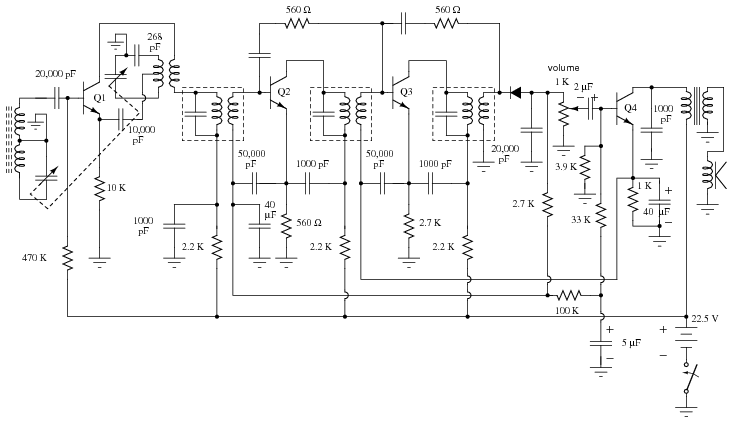
\includegraphics[width=\imgwidth]{radio_circuit.png}
\caption{A hardware implemented radio circuit}
\label{radio_circuit}
\centrefigureend

\centrefigurestart
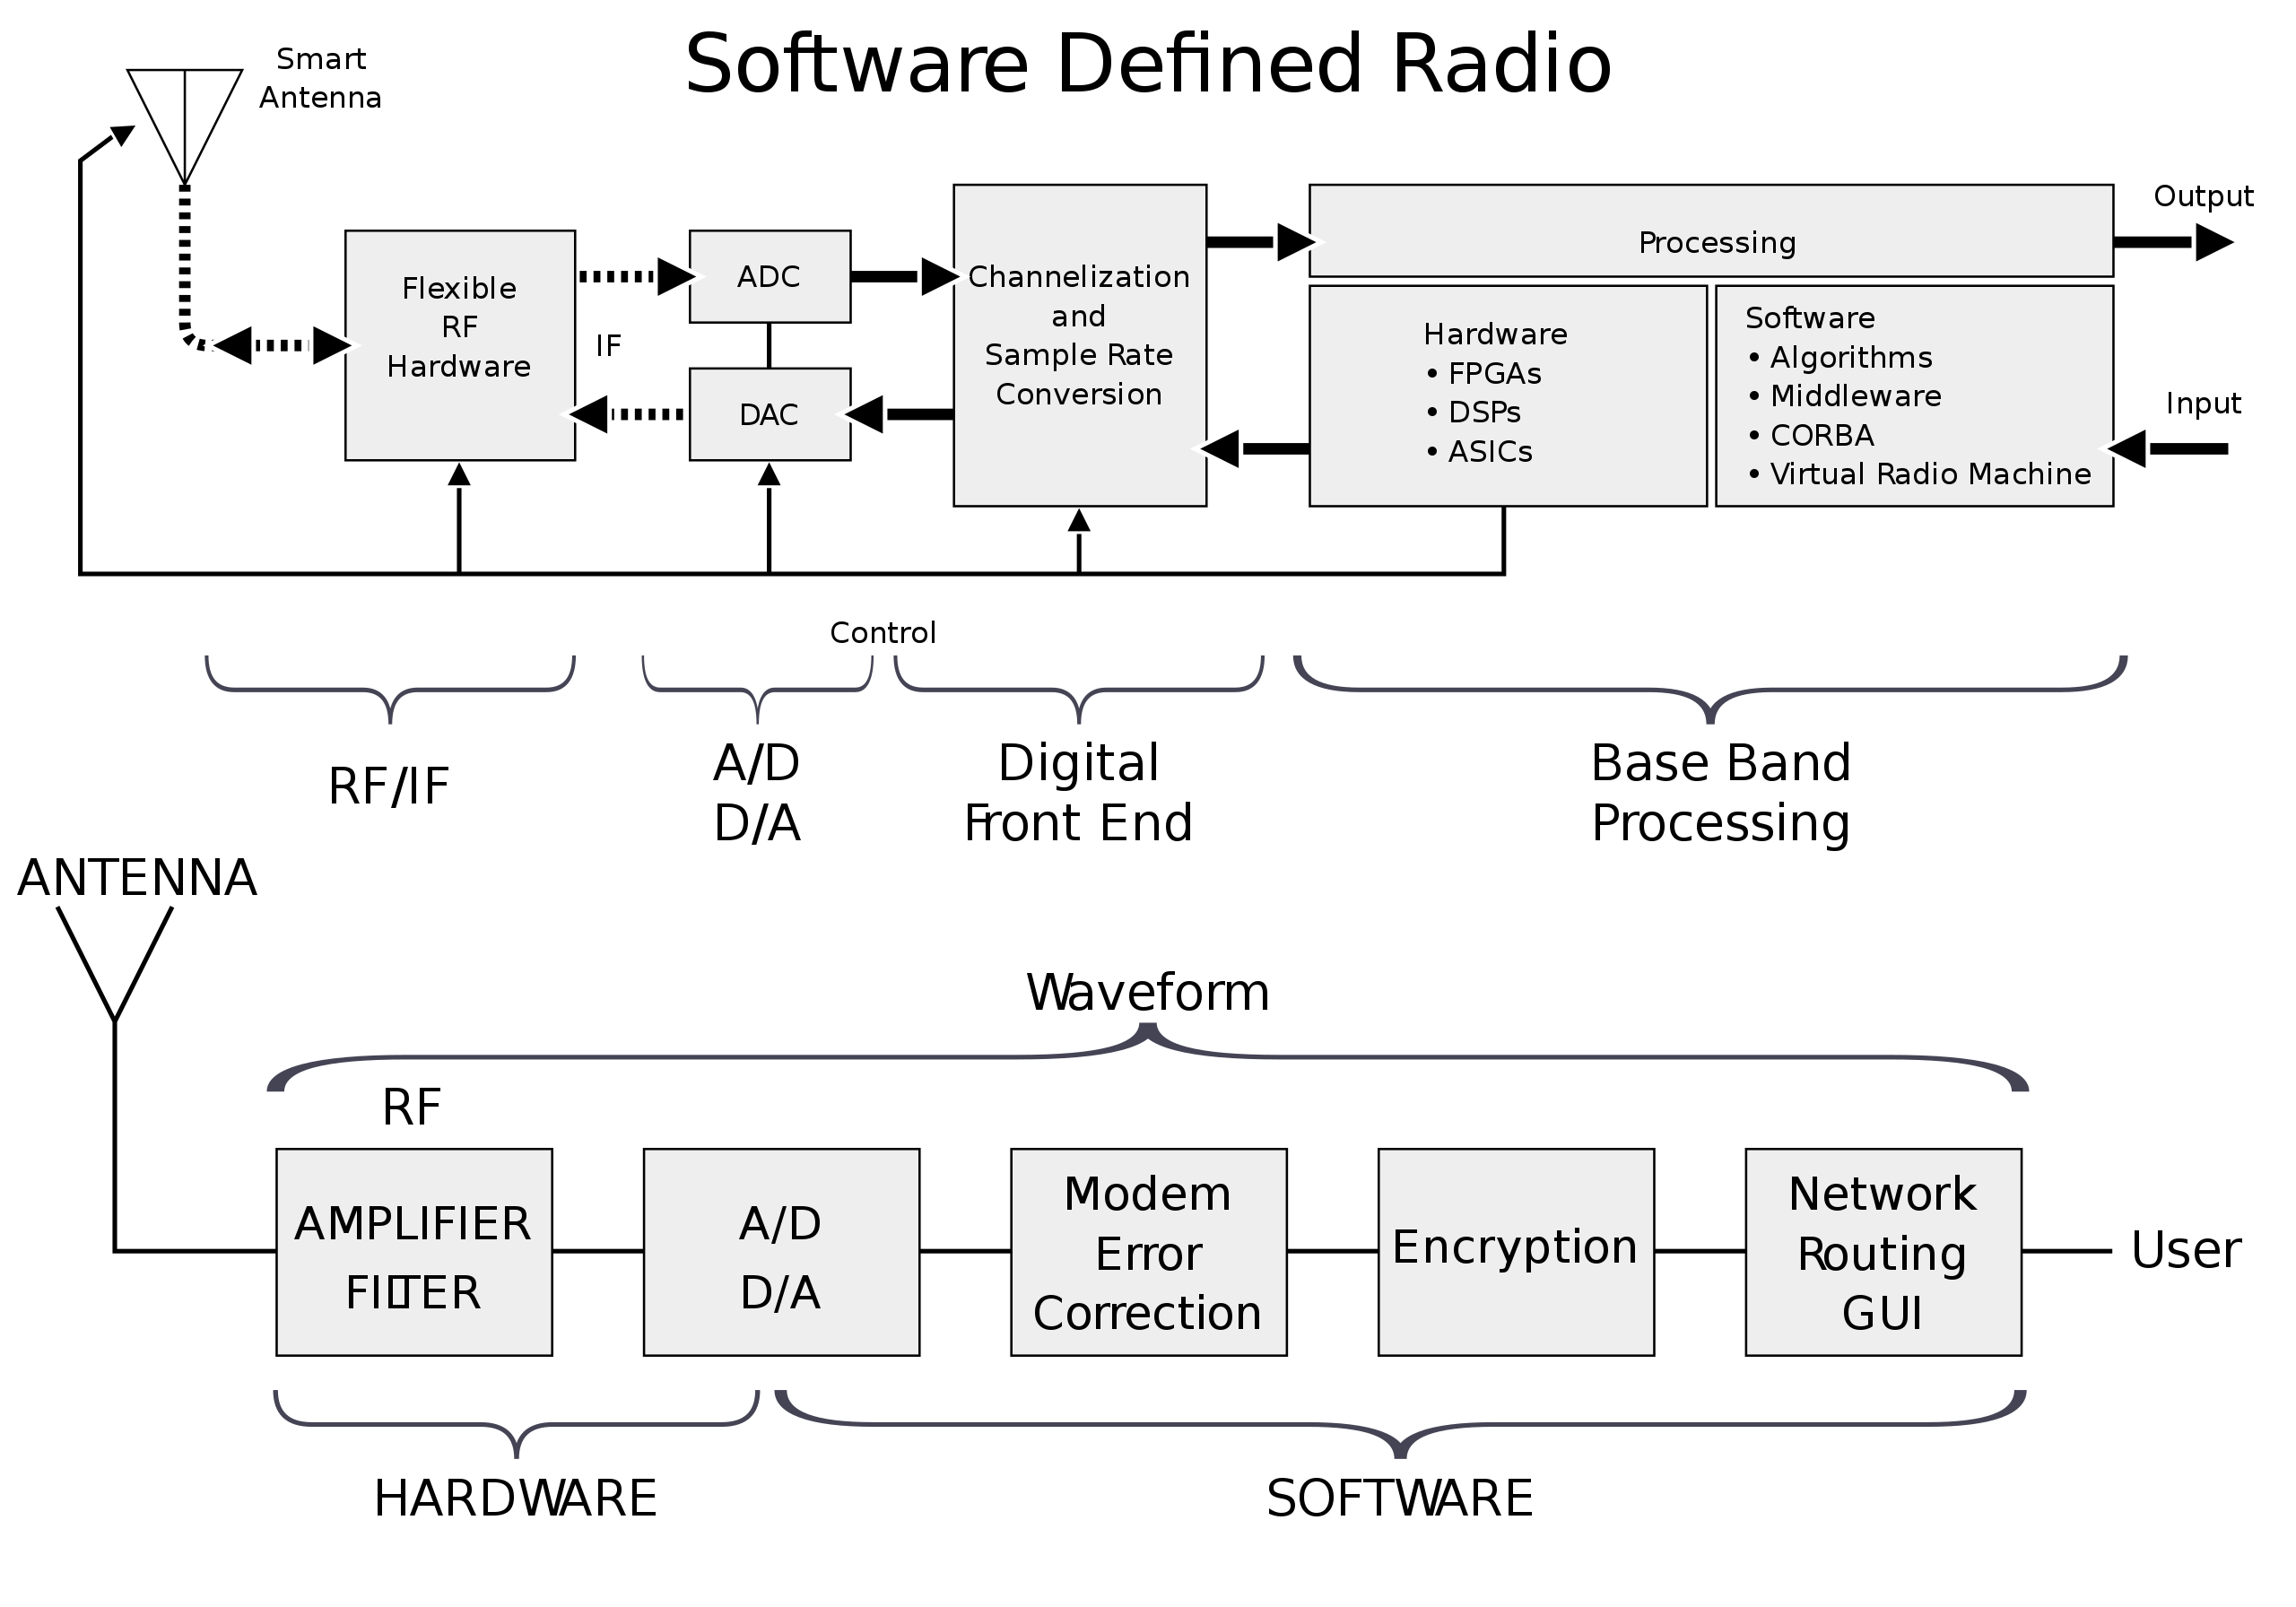
\includegraphics[width=\imgwidth]{sdr_arch.png}
\caption{A generic SDR block diagram.}
\label{sdr_arch}
\centrefigureend

\subsection{gnuradio}
This is a piece of software which provides a drag and drop \gls{gui} for performing our \gls{sdr} reconfiguration. We can also process the data after it's been received using special blocks.

\subsection{RadioHead-Extras repo}
This is a well known repository for programatically configuring an \gls{RF} transceiver chip, such as the one on the Feather module we will be using. This library is specific to the project as I have added some functionality to help us to send data without lots of extra features which will complicate things.
